\documentclass[]{elsarticle} %review=doublespace preprint=single 5p=2 column
%%% Begin My package additions %%%%%%%%%%%%%%%%%%%

\usepackage[hyphens]{url}

  \journal{Data Mining} % Sets Journal name

\usepackage{lineno} % add

\usepackage{graphicx}
%%%%%%%%%%%%%%%% end my additions to header

\usepackage[T1]{fontenc}
\usepackage{lmodern}
\usepackage{amssymb,amsmath}
\usepackage{ifxetex,ifluatex}
\usepackage{fixltx2e} % provides \textsubscript
% use upquote if available, for straight quotes in verbatim environments
\IfFileExists{upquote.sty}{\usepackage{upquote}}{}
\ifnum 0\ifxetex 1\fi\ifluatex 1\fi=0 % if pdftex
  \usepackage[utf8]{inputenc}
\else % if luatex or xelatex
  \usepackage{fontspec}
  \ifxetex
    \usepackage{xltxtra,xunicode}
  \fi
  \defaultfontfeatures{Mapping=tex-text,Scale=MatchLowercase}
  \newcommand{\euro}{€}
\fi
% use microtype if available
\IfFileExists{microtype.sty}{\usepackage{microtype}}{}
\usepackage[]{natbib}
\bibliographystyle{plainnat}

\usepackage{graphicx}
\ifxetex
  \usepackage[setpagesize=false, % page size defined by xetex
              unicode=false, % unicode breaks when used with xetex
              xetex]{hyperref}
\else
  \usepackage[unicode=true]{hyperref}
\fi
\hypersetup{breaklinks=true,
            bookmarks=true,
            pdfauthor={},
            pdftitle={ Actividad Evaluativa \#2 Grupo 5 Universidad Andrés Bello Facultad de Ingeniería Ingeniería Civil Informática Ingeniería Civil Industrial},
            colorlinks=false,
            urlcolor=blue,
            linkcolor=magenta,
            pdfborder={0 0 0}}

\setcounter{secnumdepth}{0}
% Pandoc toggle for numbering sections (defaults to be off)
\setcounter{secnumdepth}{0}


% tightlist command for lists without linebreak
\providecommand{\tightlist}{%
  \setlength{\itemsep}{0pt}\setlength{\parskip}{0pt}}



\usepackage{float}
\usepackage{booktabs}
\usepackage{longtable}
\usepackage{array}
\usepackage{multirow}
\usepackage{wrapfig}
\usepackage{float}
\usepackage{colortbl}
\usepackage{pdflscape}
\usepackage{tabu}
\usepackage{threeparttable}
\usepackage{threeparttablex}
\usepackage[normalem]{ulem}
\usepackage{makecell}
\usepackage{xcolor}



\begin{document}


\begin{frontmatter}

  \title{
\includegraphics[width=1.5625in,height=1.5625in]{logo_UNAB.png}\\
Actividad Evaluativa \#2\\
Grupo 5\\
Universidad Andrés Bello\\
Facultad de Ingeniería\\
Ingeniería Civil Informática\\
Ingeniería Civil Industrial}
    \author[]{Martín Fernández 1%
  %
  \fnref{1}}
   \ead{nombre@uandresbello.edu} 
    \author[]{Tomás Moya 2}
   \ead{nombre@uandresbello.edu} 
    \author[]{Wesly Ocampo 3%
  %
  \fnref{2}}
   \ead{nombre@uandresbello.edu} 
    \author[]{Alan Tovar 4%
  %
  \fnref{3}}
   \ead{nombre@uandresbello.edu} 
      \cortext[cor1]{Corresponding author}
  
  \begin{abstract}
  Describir brevemente en qué consiste este primer análisis de los
  datos, e incluir el objetivo del estudio. (máximo 150 palabras)
  \end{abstract}
  
 \end{frontmatter}

\newpage

\section{Introducción}

En el presente informe se presentan los resultados de un análisis de dos
modelos de regresión lineal múltiple con el objetivo de reducir las
variables no significativas y trabajar con una base de datos más
pequeña.

La reducción de dimensionalidad es la forma de convertir un conjunto de
datos de dimensiones elevadas en un conjunto de datos de dimensiones
menores, asegurando que la información que proporciona es similar en
ambos casos. Esta técnica nos permite obtener un modelo predictivo más
ajustado mientras se resuelven los problemas de regresión y
clasificación que presentan los algoritmos.

Por otro lado, la regresión logística resulta útil para los casos en los
que se desea predecir la presencia o ausencia de una característica o
resultado según los valores de un conjunto de predictores. Es similar a
un modelo de regresión lineal pero está adaptado para modelos en los que
la variable dependiente es dicotómica, es decir que puede tomar solo dos
valores. Los coeficientes de regresión logística pueden utilizarse para
estimar la razón de probabilidad de cada variable independiente del
modelo. La regresión logística se puede aplicar a un rango más amplio de
situaciones de investigación que el análisis discriminante.

\newpage
\section{Desarrollo}
\subsection{Análisis de Componentes}

Para el análisis de componentes principales no tomamos en cuenta la
variable cantidad de bicicletas rentadas ya que corresponde a la
variable dependiente y eliminando las variables categóricas dejando
únicamente las variables numéricos, obteniendo un total de 10 variables,
observando el gráfico de proporción de varianzas a la izquierda podemos
ver que tiene porcentajes bastante disparejos presentando una diferencia
de porcentajes de alrededor del 27\% entre el primer y último
componente, según el gráfico de varianza acumulada con 4 componentes se
puede lograr el 70\% de la variabilidad total de los datos.

\begin{figure}[H]

{\centering 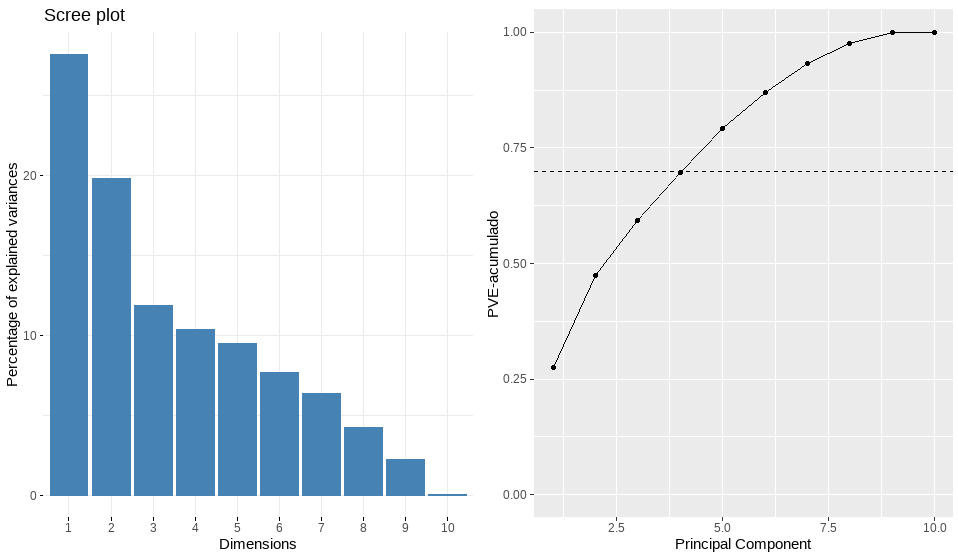
\includegraphics[width=1\linewidth]{cp1} 

}

\caption{\label{fig:fig1}Análisis de Componentes.}\label{fig:fig1}
\end{figure}

En el gráfico de contribución de cada variable podemos observar que en
las 2 primeras dimensiones tenemos un total del 47,5\% de la
variabilidad total de los datos, dentro de la dimensión 1 los
componentes que contribuyen significativamente de forma positiva son
radiación solar con gran contribución, mientras que en menor medida
Hora, velocidad del viento, visibilidad y temperatura. De forma negativa
en la dimensión 1 serian humedad con gran contribución y en menor
contribución serian lluvia y nevada. En la dimensión 2 los componentes
que contribuyen significativamente de forma positiva temperatura de
punto de rocío y temperatura con gran contribución y en menor
contribución, humedad y lluvia. De forma negativa en la dimensión 2
serian nevada y visibilidad con poca contribución

\begin{figure}[H]

{\centering 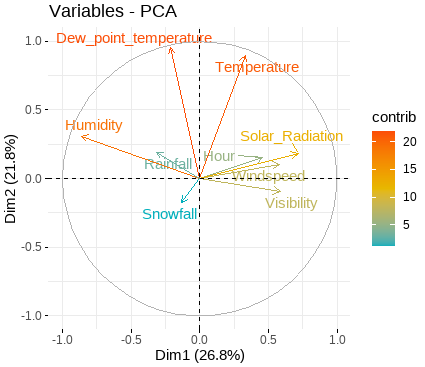
\includegraphics[width=1\linewidth]{cp2} 

}

\caption{\label{fig:fig2}Análisis de Componentes.}\label{fig:fig2}
\end{figure}

\newpage
\subsection{Regresión Lineal Múltiple.}
\subsection{Modelo 1.}
\begin{table}

\caption{\label{tab:tab1}\label{tab:tab1}Modelo 1.}
\centering
\begin{tabular}[t]{l|l|r|r|r|r}
\hline
  & Variables & Estimación & Std.Error & t.value & P-valor\\
\hline
(Intercept) & (Intercept) & 862.41 & 143.67 & 6.00 & 0.00\\
\hline
Hour & Hour & 39.27 & 1.22 & 32.27 & 0.00\\
\hline
Temperature & Temperature & 16.48 & 5.64 & 2.92 & 0.00\\
\hline
Humidity & Humidity & -12.22 & 1.57 & -7.76 & 0.00\\
\hline
Windspeed & Windspeed & 23.55 & 8.85 & 2.66 & 0.01\\
\hline
Visibility & Visibility & 0.00 & 0.02 & 0.16 & 0.87\\
\hline
Dew\_point\_temperature & Dew\_point\_temperature & 6.07 & 5.80 & 1.05 & 0.30\\
\hline
Solar\_Radiation & Solar\_Radiation & -108.85 & 11.44 & -9.52 & 0.00\\
\hline
Rainfall & Rainfall & -55.82 & 6.08 & -9.19 & 0.00\\
\hline
Snowfall & Snowfall & -2.48 & 24.79 & -0.10 & 0.92\\
\hline
\end{tabular}
\end{table}

Para el primer modelo podemos ver como las variables Visibility,
Dew\_point\_temperature y Snowfall no son significativas ya que su
p-valor es mayor a 0.05 o 5\%.

\begin{figure}[H]

{\centering 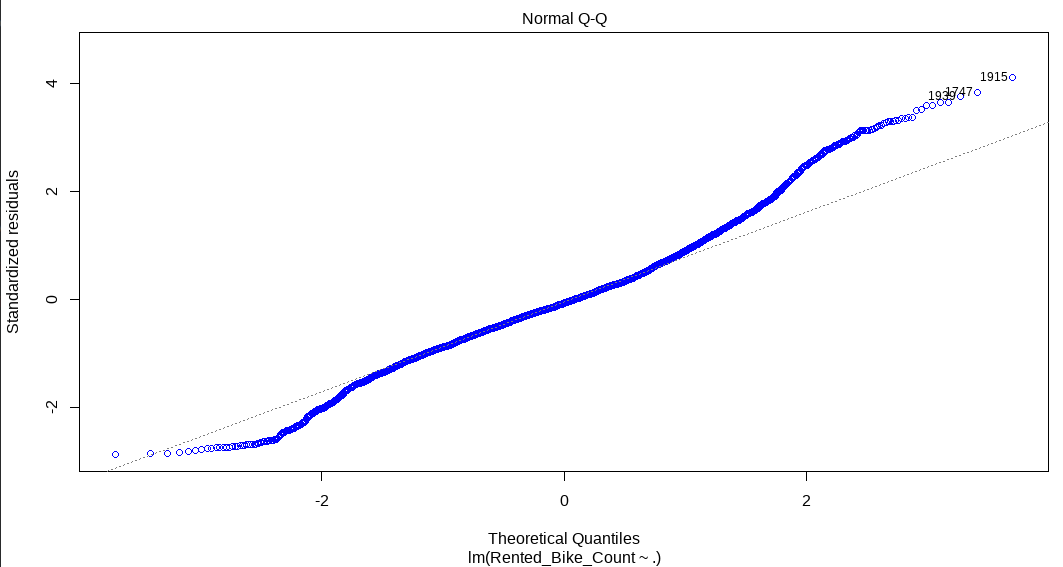
\includegraphics[width=1\linewidth]{qq} 

}

\caption{\label{fig:fig3} Q-Q plot Modelo 1.}\label{fig:fig3}
\end{figure}

\begin{figure}[H]

{\centering 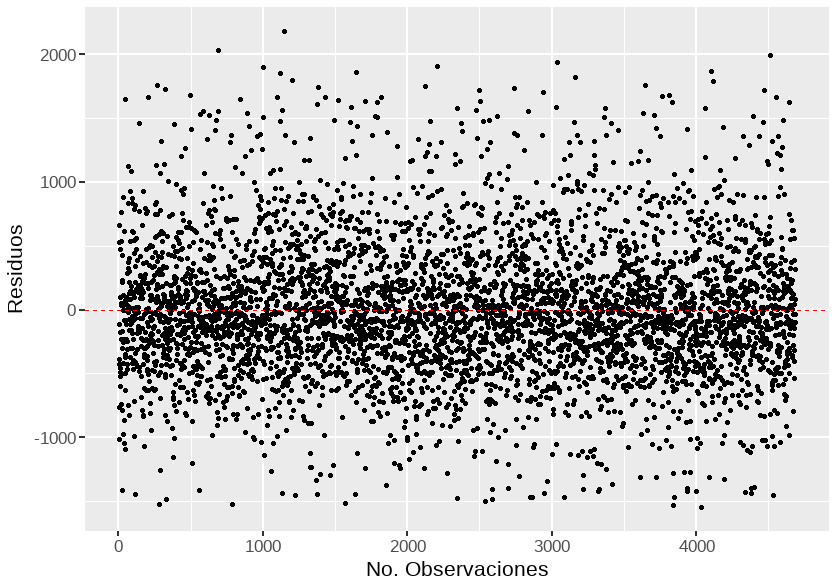
\includegraphics[width=1\linewidth]{resid} 

}

\caption{\label{fig:fig4} Residuos Modelo 1.}\label{fig:fig4}
\end{figure}

\begin{verbatim}
## 
##  Shapiro-Wilk normality test
## 
## data:  dat.train$resid
## W = 0.97858, p-value < 2.2e-16
\end{verbatim}

Además no se cumplen los supuestos de normalidad.

\newpage
\subsection{Modelo 2.}

\begin{table}

\caption{\label{tab:tab2}\label{tab:tab2}Modelo 2.}
\centering
\begin{tabular}[t]{l|l|r|r|r|r}
\hline
  & Variables & Estimación & Std.Error & t.value & P-valor\\
\hline
(Intercept) & (Intercept) & 733.12 & 41.70 & 17.58 & 0.00\\
\hline
Hour & Hour & 39.18 & 1.21 & 32.38 & 0.00\\
\hline
Temperature & Temperature & 22.36 & 1.03 & 21.70 & 0.00\\
\hline
Humidity & Humidity & -10.76 & 0.50 & -21.54 & 0.00\\
\hline
Windspeed & Windspeed & 23.14 & 8.84 & 2.62 & 0.01\\
\hline
Solar\_Radiation & Solar\_Radiation & -112.11 & 10.81 & -10.37 & 0.00\\
\hline
Rainfall & Rainfall & -56.67 & 6.01 & -9.43 & 0.00\\
\hline
\end{tabular}
\end{table}

Para este modelo 2 todas nuestras variables son significativas.

\newpage
\subsection{Comparación de Modelos.}
\begin{table}

\caption{\label{tab:tab3}\label{tab:tab3}Medidas de Comparación de los Modelos.}
\centering
\begin{tabular}[t]{l|r|r}
\hline
Medidas & Modelo\_1 & Modelo\_2\\
\hline
R2.ajustado & 41.12 & 41.15\\
\hline
COR & 0.63 & 0.63\\
\hline
BIAS & -1.31 & -1.49\\
\hline
RMSE & 532.97 & 532.82\\
\hline
\end{tabular}
\end{table}

R cuadrado ajustado nos indica el porcentaje de variabilidad total de la
variable de respuesta, en este caso no hay una gran diferencia pero el
modelo 2 explica en un 41,14\% el índice de bicicletas rentadas, es
decir un 0.02\% más que el modelo 1. Por otro lado la medida cor nos
indica la correlación entre lo predicho y lo observado, es decir entre
más cercano a 1 sea es mejor, por lo que igual que en el punto anterior
el dos es mejor.

El promedio del error (BIAS), nos indica la relación entre el error
esperado y el obtenido, aquí al obtener valor negativo nos indica que
obtuvimos un valor mayor al esperado. Y el error cuadrático medio RMSE
indica que entre menor sea su valor es mejor nuestro modelo, y en este
caso nuevamente el segundo modelo es mejor que el primero.

\begin{figure}[H]

{\centering 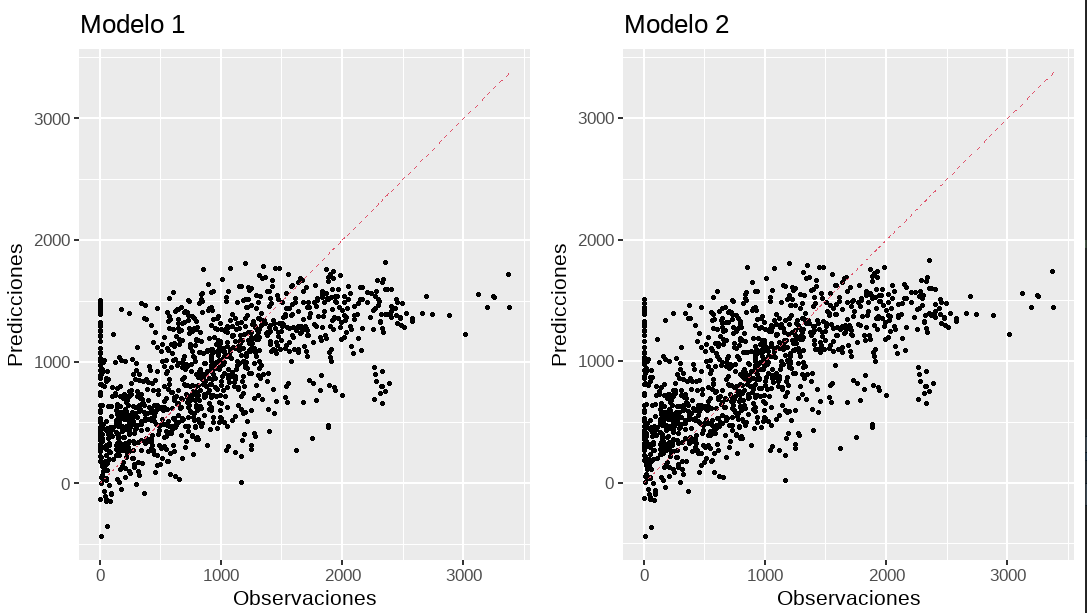
\includegraphics[width=1\linewidth]{compare_g} 

}

\caption{\label{fig:fig5} Comparación de los Modelos.}\label{fig:fig5}
\end{figure}

\newpage
\section{Conclusiones}

Luego de este análisis podemos concluir que los modelos son similares y
no son viables. Esto se debe a que la variable dependiente con la que
trabajamos (Bicicletas rentadas) tiene una distribucion asimetrica
positiva, por la regresion lineal multiple no arroja un buen modelo,
para obtener un modelo viable tendríamos que convertir la variable para
que tenga una distribución normal y luego realizar nuevamente la
regresión.


\end{document}
